\documentclass[letterpaper,11pt]{article}
\oddsidemargin -1.0cm \textwidth 17.5cm

\usepackage[utf8]{inputenc}
\usepackage[activeacute,spanish, es-lcroman]{babel}
\decimalpoint
\usepackage{amsfonts,setspace}
\usepackage{amsmath}
\usepackage{amssymb, amsmath, amsthm}
\usepackage{comment}
\usepackage{float}
\usepackage{amssymb}
\usepackage{dsfont}
\usepackage{anysize}
\usepackage{multicol}
\usepackage{enumerate}
\usepackage{graphicx}
\usepackage[left=1.5cm,top=2cm,right=1.5cm, bottom=1.7cm]{geometry}
\setlength\headheight{1.5em} 
\usepackage{fancyhdr}
\usepackage{multicol}
\usepackage{hyperref}
\usepackage{wrapfig}
\usepackage{subcaption}
\usepackage{siunitx}
\usepackage{cancel}
\usepackage{mdwlist}
\usepackage{svg}
\pagestyle{fancy}
\fancyhf{}
\renewcommand{\labelenumi}{\normalsize\bfseries P\arabic{enumi}.}
\renewcommand{\labelenumii}{\normalsize\bfseries (\alph{enumii})}
\renewcommand{\labelenumiii}{\normalsize\bfseries \roman{enumiii})}


\begin{document}

\fancyhead[L]{\itshape{Facultad de Ciencias F\'isicas y Matem\'aticas}}
\fancyhead[R]{\itshape{Universidad de Chile}}

\begin{minipage}{11.5cm}
    \begin{flushleft}
        \hspace*{-0.6cm}\textbf{FI1000-1 Introducción a la Física Clásica}\\
        \hspace*{-0.6cm}\textbf{Profesor:} Ignacio Bordeu\\
        \hspace*{-0.6cm}\textbf{Auxiliares:} Javier Cubillos \& Berenice Muruaga\\
        \hspace*{-0.6cm}\textbf{Auxiliares taller:} Pablo González \& Alejandro Cartes\\
        \hspace*{-0.6cm}\textbf{Ayudante:} Amaru Moya\\
    \end{flushleft}
\end{minipage}

\begin{picture}(2,3)
    \put(366, 10){
\includegraphics[scale=0.9]{2020-1/Imágenes/logo/dfi-fcfm.pdf}}
\end{picture}

\begin{center}
	\LARGE\textbf{Taller \#4}\\
	\Large{Movimiento Relativo, MCU y Cinemática}
\end{center}

\vspace{-1cm}
\begin{enumerate}\setlength{\itemsep}{0.4cm}\addtocounter{enumi}{-0}

\rfoot[]{pág. \thepage}

\item[]

\item \textbf{(Movimiento Relativo)} Un piloto debe volar su avión hacia el norte para llegar a su destino. El avión puede volar a $300 \frac{km}{h}$ en aire en calma. Un viento sopla del noreste (a $45^\circ$) a $90 \frac{km}{h}$.

\begin{enumerate}
    \item ¿Cuál es la rapidez del avión con respecto al suelo, en metros por segundo?
    
    \item ¿En qué dirección debe dirigir su avión el piloto para volar directamente hacia el norte?
    
\end{enumerate}

\item (\textbf{MCU - mov. parabólico})

\begin{multicols}{2}
     Imagine un mundo que transcurre sobre una plataforma circular de radio muy grande, que gira con velocidad angular $\Omega$ constante. En el entorno de la plataforma existe una aceleración de gravedad $\vec{g}$ constante. Una persona ubicada a una distancia $L$ del centro $O$, en reposo con respecto a la plataforma, lanza una moneda al aire en dirección vertical y con rapidez $v_0$ (respecto a la persona). 
    \columnbreak
    
    \begin{figure}[H]
        \centering
        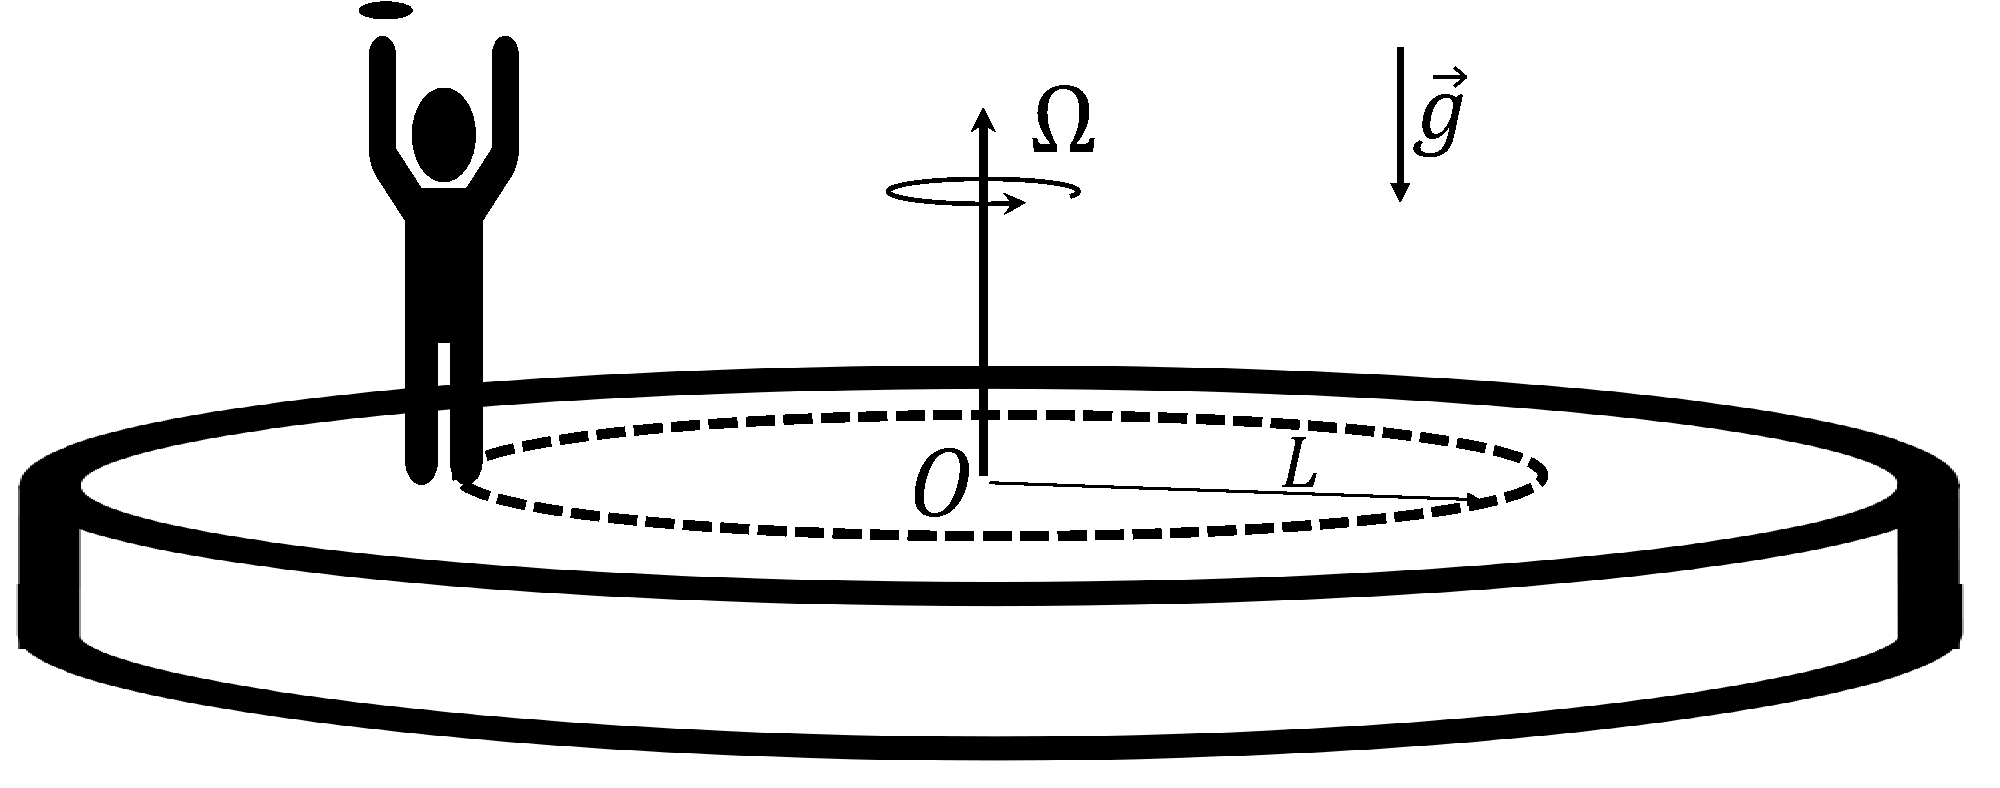
\includegraphics[width = 0.8\linewidth]{2021-1/Imagenes/aux4/moneda-circulo.pdf}
    \end{figure}
\end{multicols}

Determine el tiempo que demora en caer la moneda al suelo y el lugar sobre la plataforma, con respecto a la persona, donde lo hace.
\textbf{\textit{Hint:}} Analice el lanzamiento de la moneda desde un observador ubicado en un sistema $S$ fijo con origen en $O$


\item \textbf{(Cinemática 1D)} Una fila de soldados de largo $L$ marcha en líınea recta, uno detrás de otro. Un oficial recorre la columna, comenzando desde el último soldado, con rapidez constante $U$. En el instante que alcanza la cabeza de la columna, se devuelve con la misma rapidez, hasta que se encuentra con el último soldado de la columna. Durante este intervalo la columna de soldados ha permanecido en movimiento con rapidez constante $V$ y se ha desplazado una distancia $L$ desde el instante en que el oficial comenzó a adelantarse en la columna. De esta forma, el último soldado se encuentra en el lugar donde estuvo el primer soldado en el instante en que el oficial se dispuso a revisar la tropa.

\begin{enumerate}
    \item Dibuje un esquema de la situación
    \item Haga un gráfico con las posiciones del oficial y del último soldado de la fila en función del tiempo
    \item ¿Qué distancia total recorrió el oficial?
    \item Encuentre la razón entre los valores de $U$ y $V$
\end{enumerate}


% Para imágenes vectoriales -> el texto tiene que estar en LaTeX
% \begin{figure}[htbp]
%   \centering
%   \svgpath{../Imagenes/ejercicios}  -> .. irse pa'trás 
%   \includesvg{ej5.svg}
% \end{figure}

\end{enumerate}
\end{document}
